\begin{figure}[htbp]

\centering
\begin{subfigure}[t]{0.49\textwidth}
\captionsetup{labelformat=empty}

\caption{\textbf{AAPL}}
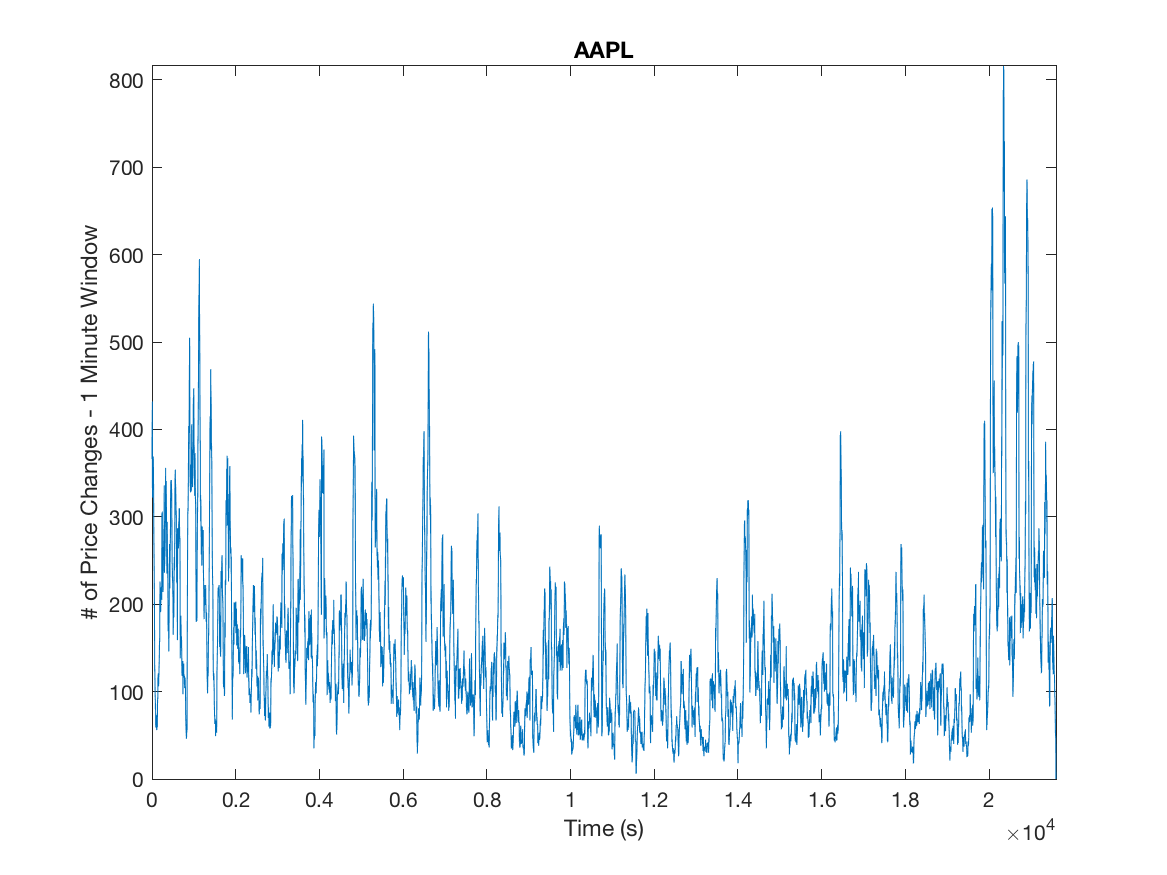
\includegraphics[width=\textwidth, trim = 0 0 0 30, clip]{Cluster_Plots/AAPL_cluster.png}

\end{subfigure}
\begin{subfigure}[t]{0.49\textwidth}
\captionsetup{labelformat=empty}

\caption{\textbf{AMZN}}
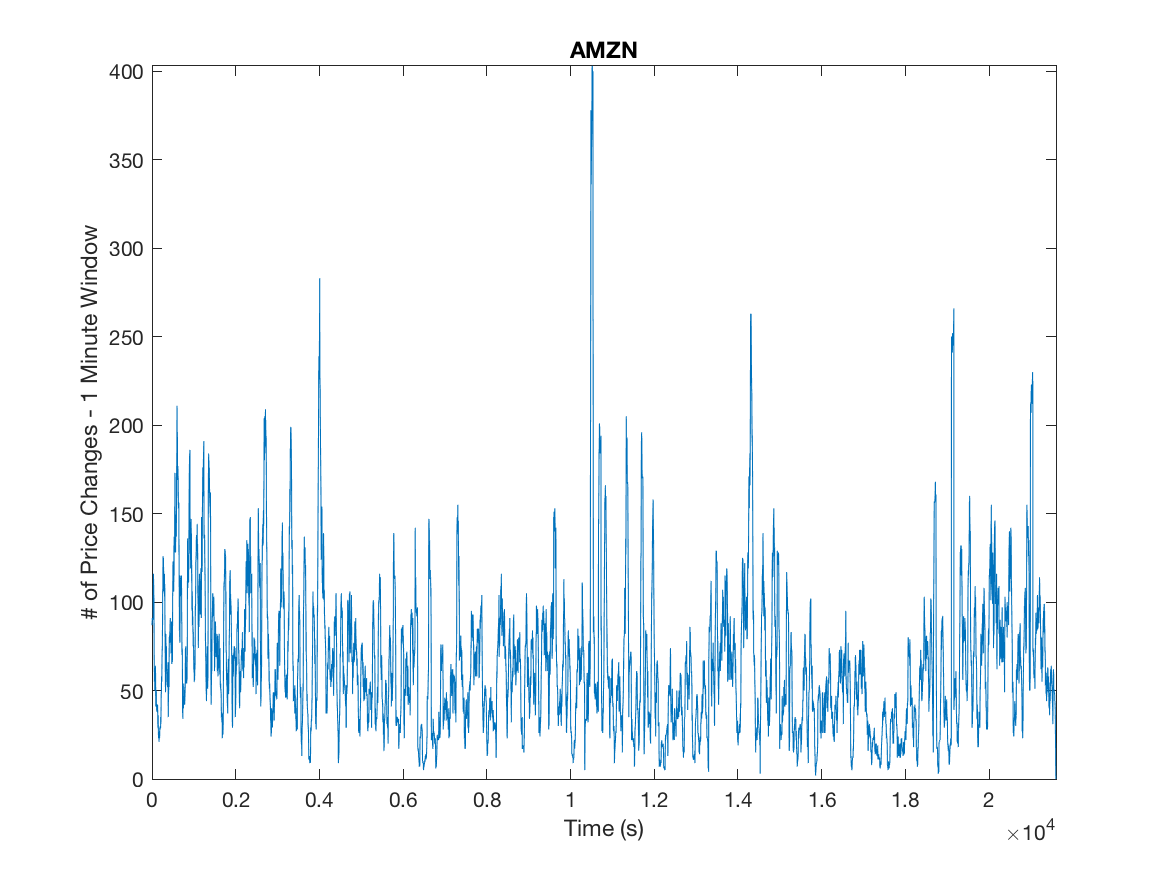
\includegraphics[width=\textwidth, trim = 0 0 0 30, clip]{Cluster_Plots/AMZN_cluster.png}
\end{subfigure}

\vspace{3mm}

\begin{subfigure}[t]{0.49\textwidth}
\captionsetup{labelformat=empty}

\caption{\textbf{GOOG}}
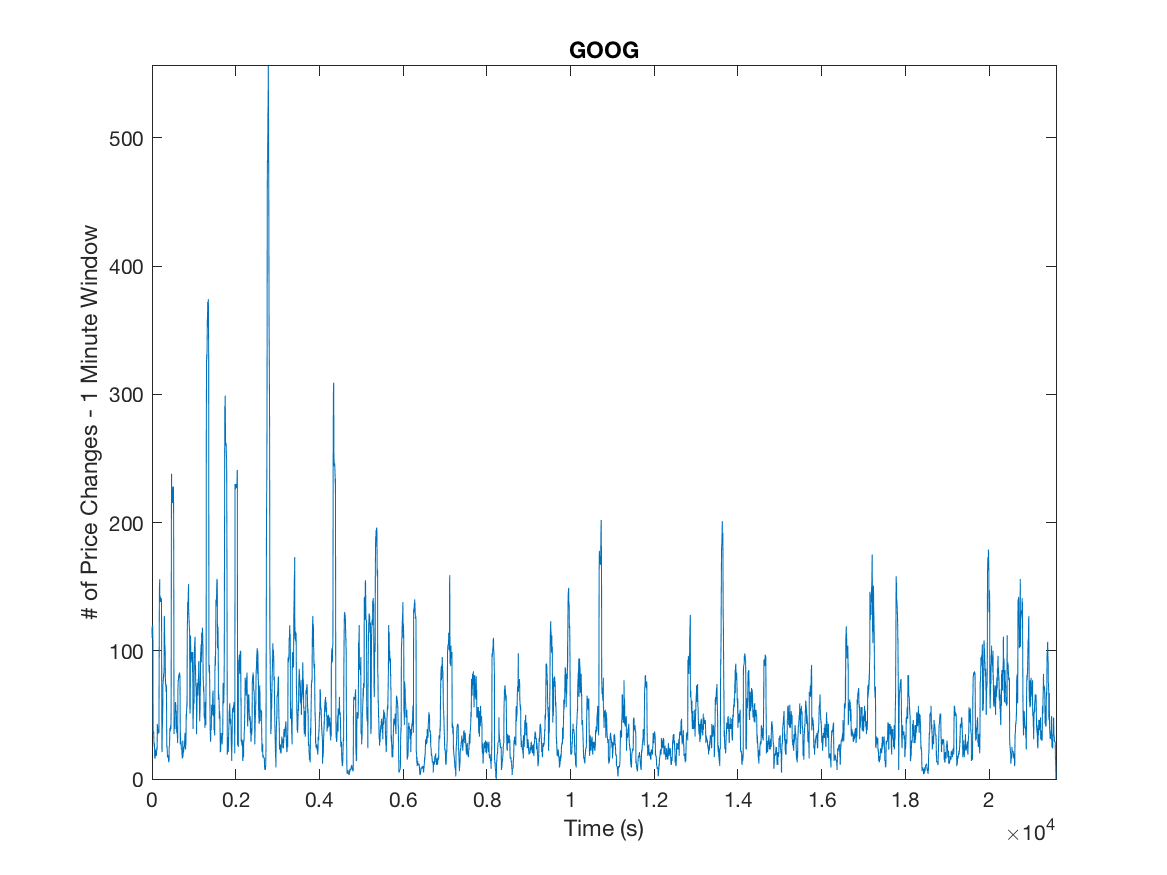
\includegraphics[width=\textwidth, trim = 0 0 0 30, clip]{Cluster_Plots/GOOG_cluster.png}

\end{subfigure}
\begin{subfigure}[t]{0.49\textwidth}
\captionsetup{labelformat=empty}

\caption{\textbf{INTC}}
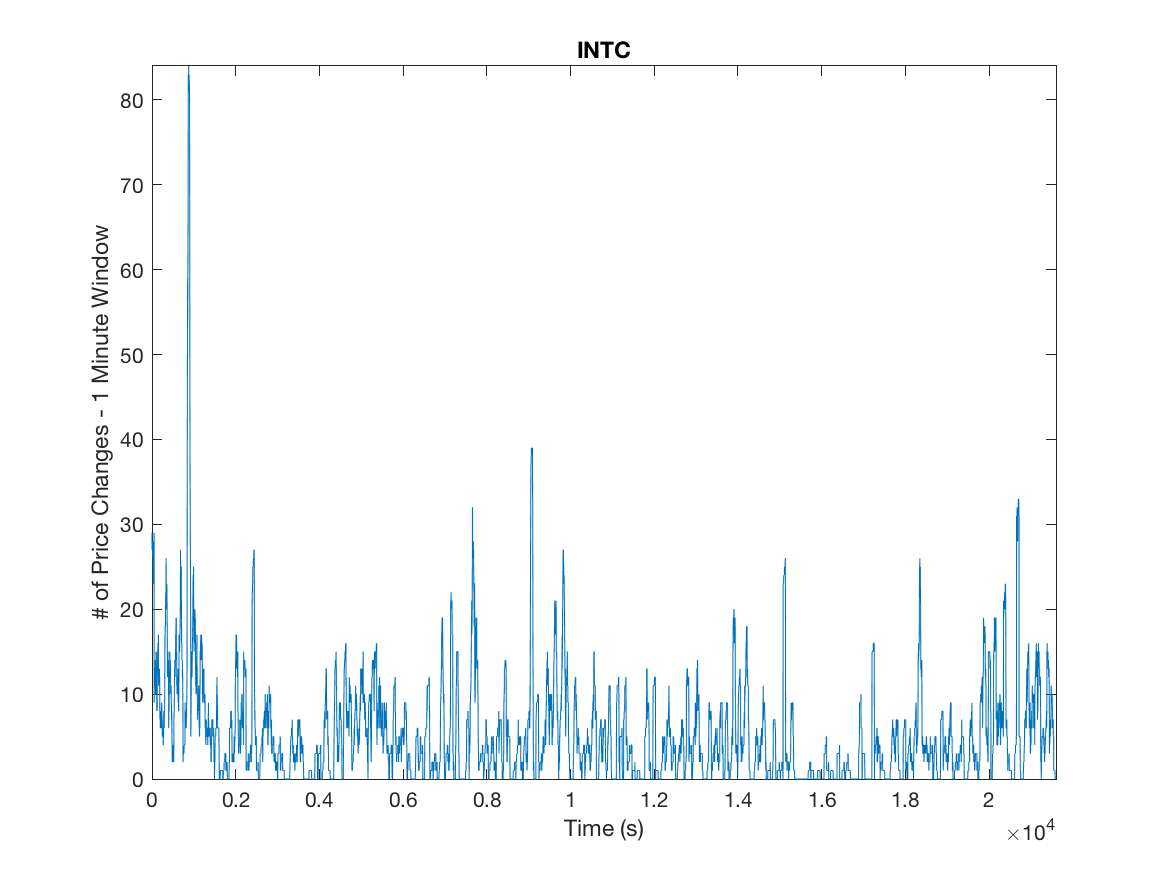
\includegraphics[width=\textwidth, trim = 0 0 0 30, clip]{Cluster_Plots/INTC_cluster.png}
\end{subfigure}

\vspace{3mm}

\begin{subfigure}[t]{0.49\textwidth}
\captionsetup{labelformat=empty}

\caption{MSFT}
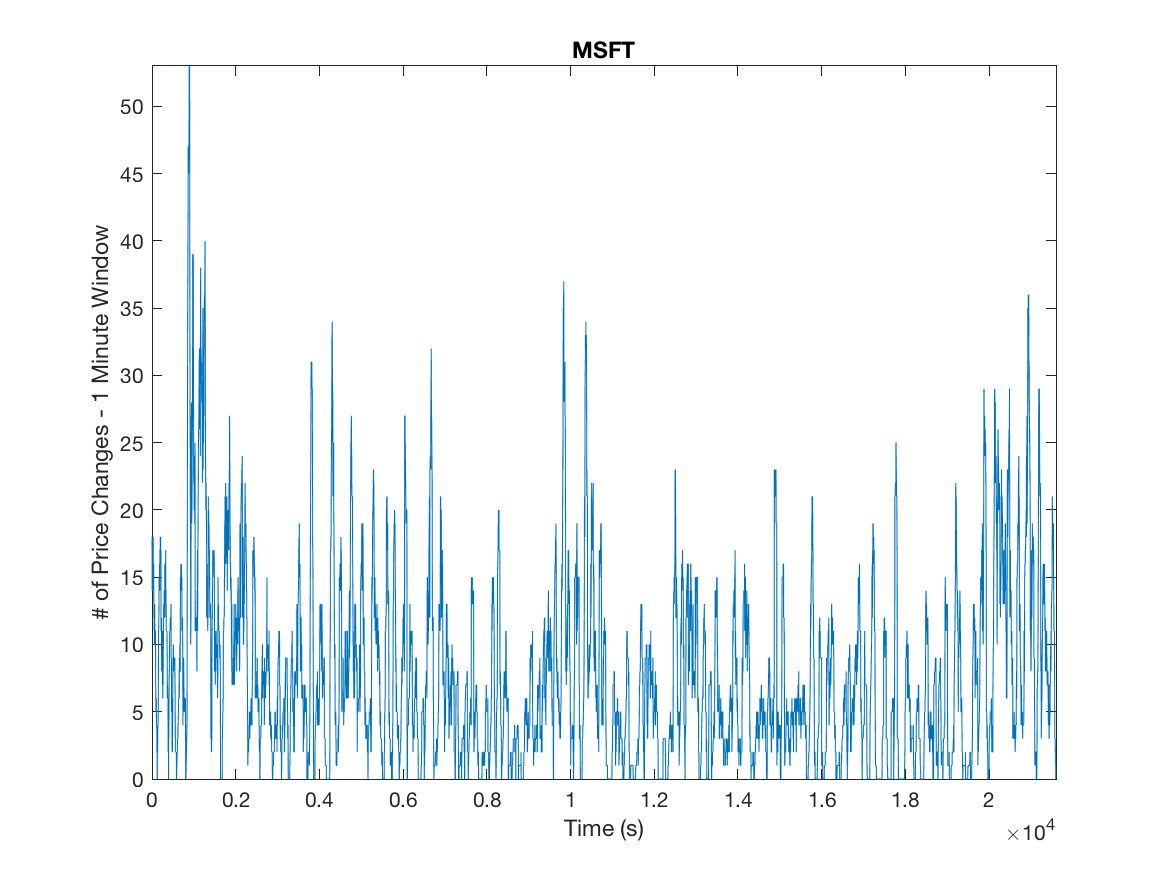
\includegraphics[width=\textwidth, trim = 0 0 0 30, clip]{Cluster_Plots/MSFT_cluster.png}
\end{subfigure}

\caption{\label{fig:clustering} Each plot shows the number of arrivals for a moving one minute window. From this we can conclude that there is a significant amount of clustering in the arrival of mid price changes, motivating the Hawkes model of our arrival process.}
\end{figure}